\chapter{Overview of the $\text{M}_\text{T2}$ Analysis}

\section{Motivation for an all-hadronic search}

\section{Sources of backgrounds}

\begin{figure}[h]
  \begin{center}
    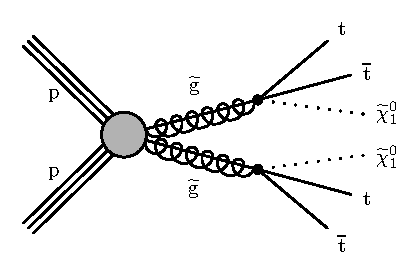
\includegraphics[width=0.40\textwidth]{figs/susy_diagrams/T1tttt.pdf}
    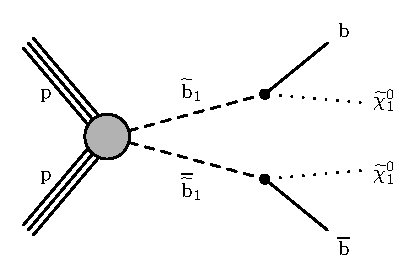
\includegraphics[width=0.40\textwidth]{figs/susy_diagrams/T2bb.pdf}
    \caption{Example Feynman diagrams of strongly-produced SUSY particles decaying hadronically.
      (left) Gluino pair production, where each gluino decays into a neutralino and two top quarks.
      (right) Bottom squark pair production, where each squark decays into a neutralino and bottom quark.
            }
    \label{Fig:example_susy_feyn}
  \end{center}
\end{figure}


\section{The $M_\text{T2}$ variable}

Defining the \emph{transverse energy} of a particle as $E_\mrm{T}^2\equiv m^2+\pt^2$, we can define the \emph{transverse mass} of a two-particle system as
\be\label{eq:mtlong}
\begin{split}
M_\mrm{T}^2 &\equiv (E_\mrm{T,1}+E_\mrm{T,2})^2 - (\vec{p}_\mrm{T,1} + \vec{p}_\mrm{T,2})^2 \\
&= m_1^2 + m_2^2 + 2(E_\mrm{T,1}E_\mrm{T,2} - \vec{p}_\mrm{T,1}\cdot\vec{p}_\mrm{T,2}).
\end{split}
\ee

Assuming massless particles (or, equivalently, particles that are highly relativistic such that $E\gg m$ and $E_\mrm{T}\approx\pt$), this simplifies to
\be\label{eq:mt}
M_\mrm{T}^2 = 2p_\mrm{T,1}p_\mrm{T,2}(1-\cos\theta),
\ee
where $\theta$ is the opening angle between the particle momentum vectors.

This variable is frequently useful when a particle decays to something visible and something invisible (e.g. $W\to e\nu$).
Assuming that the invisible particle is the dominant source of missing energy in the event, the \vMet vector is approximately the
transverse momentum vector of the invisible particle and can be plugged into Eq.~\ref{eq:mt} to compute the transverse mass of the
system. As the transverse mass is just the invariant mass computed only with the transverse components of the particle momenta,
it naturally has an upper bound equal to the parent particle mass. An example from a CMS measurement of the $W$ production
cross section \cite{CMS:w_prod} is shown in Fig.~\ref{Fig:w_transverse_mass}. In this case, the two-particle system is
$W\to\mu\nu$ decay, and $M_\mrm{T}\lessapprox M_W=80~\GeV$. The location of the $M_\mrm{T}$ ``cliff'' can be used to
extract a measurement of the $W$ mass. The small number of events with transverse mass larger than the $W$ mass
are due to experimental resolution on the muon momentum and \vMet vectors.

\begin{figure}[t]
  \begin{center}
    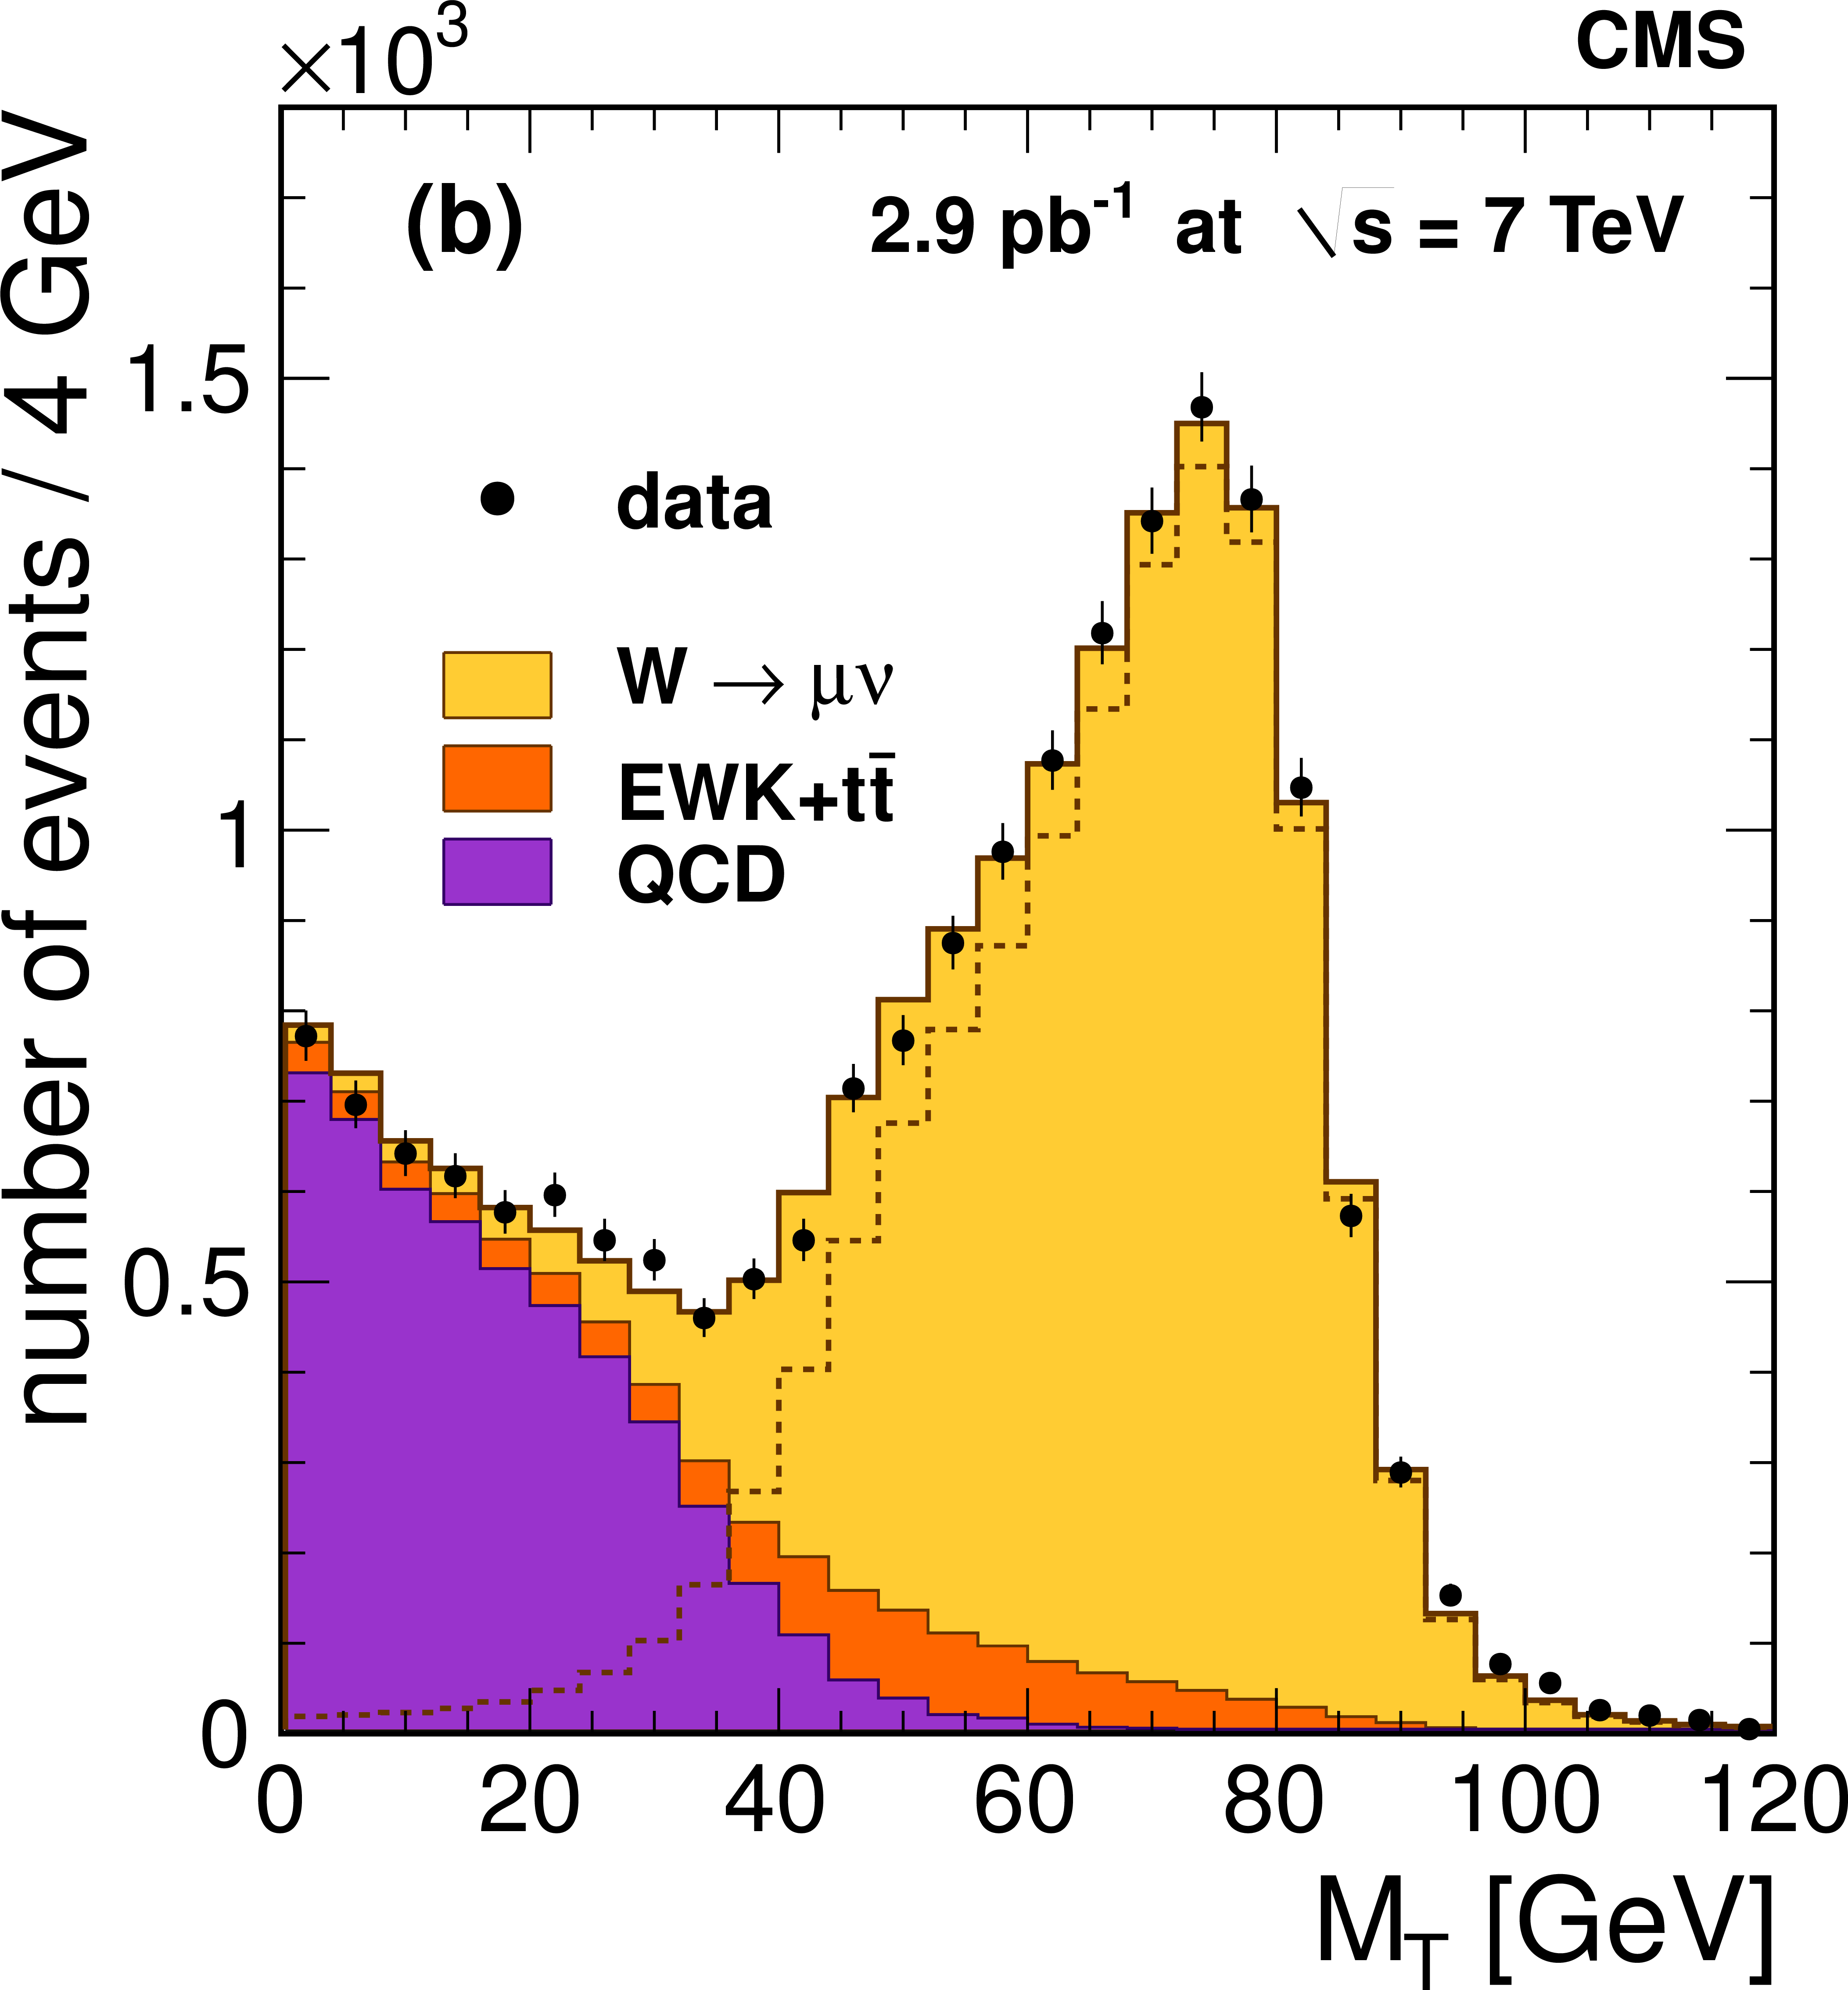
\includegraphics[width=0.45\textwidth]{figs/overview_mt2/w_transverse_mass.png}
    \caption{Transverse mass of the muon-\vMet system from a CMS measurement of the $W$ production cross section \cite{CMS:w_prod}.
      The transverse mass has a rough upper bound at $M_W=80~\GeV$, limited by experimental resolution.
            }
    \label{Fig:w_transverse_mass}
  \end{center}
\end{figure}

Computing the transverse mass of a decaying SUSY particle would be useful, since they tend to be much heavier than
SM particles that make up the background. However, the SUSY particles are \emph{pair-produced}, and computing the transverse mass 
of each system is not possible because it is not possible to resolve the \vMet vector into components from
each invisible particle. An example of this is the SUSY bottom squark pair production shown in 
Fig.~\ref{Fig:example_susy_feyn} (right). Each bottom squark decays into a b quark, which appears
as a jet in the detector (potentially b-tagged), and a neutralino, which is invisible.

Absent this information, the best we can do is to try \emph{all possible partitions} of the \vMet vector
and choose the one that gives the weakest $M_\mrm{T}$ bound. This quantity should be bounded above
by the mass of the pair-produced parent particles.
So, following \cite{mt2_def} we define
\be
\mttwo = \min_{\vSS{p}{\mrm{T}}{X(1)} + \vSS{p}{\mrm{T}}{X(2)} = \vMet}
\left[\max\left(M_\mrm{T}^{(1)},M_\mrm{T}^{(2)}\right)\right],
\ee
where (from Eq.~\ref{eq:mtlong})
\be
M_\mrm{T}^{(i)2} = m_{\mrm{vis}(i)}^2 + m_X^2 + 
2\left(E_\mrm{T}^{\mrm{vis}(i)}E_\mrm{T}^{X(i)} - \vSS{p}{\mrm{T}}{\mrm{vis}(i)}\cdot\vSS{p}{\mrm{T}}{X(i)}\right)
\;\;(i=1,2),
\ee
vis$(i)$ represents the $i^\mrm{th}$ ``visible'' system, $E_\mrm{T}^{X(i)}$ and $\vSS{p}{\mrm{T}}{X(i)}$ are the assigned transverse energy and momentum of each invisible particle, 
and $m_X$ is the mass of the invisible particle. The maximum of $M_\mrm{T}^{(1)},M_\mrm{T}^{(2)}$ is used, since if
the correct momenta are chosen then \emph{both} should be bounded above by the parent mass.

A couple of complications arise when trying to practically implement this. First, there are typically more than two visible objects
in an event (either the event is accompanied by ISR or pileup jets, or the decay cascade natrually produces more than one visible
object. For example, gluino decay into top quarks, illustrated in Fig.~\ref{Fig:example_susy_feyn} (left), produces multiple jets per
decaying gluino). If the original pair-produced particles are produced back-to back, the visible systems tend to be in opposite
hemispheres. So before computing \mttwo, all jets in the event are clustered into two \emph{pseudojets} following the algorithm
described in Ref.~\cite{CMS:tdr}, Section 13.4. First, two initial seed axes are chosen. In this analysis they are chosen
by identifying the two jets that have the largest dijet invariant mass. Next, other jets are associated to one of these axes
according to a clustering criterion. Here we use the minimal Lund distance, meaning that jet $k$ is associated to hemisphere
$i$ rather than hemisphere $j$ if
\be
(E_i-p_i\cos\theta_{ik})\frac{E_i}{(E_i+E_k)^2} < (E_j-p_j\cos\theta_{jk})\frac{E_j}{(E_j+E_k)^2}.
\ee

After all jets are associated to one or the other axis, the axes are recalculated as the sum of the
momenta of all jets connected to a hemisphere. The association is iterated using these new axes
until no jets switch from one group to the other.
